\chapter{Practical Considerations for Projection-Based Training}
\section{Architecture and Initialization}
\label{sec:arch-init}
Shallow networks are preferred in this framework, being both more stable and empirically stronger than their deeper counterparts. Equally important is maintaining a clean computational graph: every operation must either leave gradients untouched under standard Torch or be replaced by a $\mathcal{P}$
Torch equivalent. Mixing in standard Torch layers confuses targets with gradients in ways that are easy to miss. The resulting bugs are often silent; their effects only become apparent as instabilities during training

Initialization is critical as can be seen in \cref{fig:effect-of-init}; at present, the framework relies on the same initialization heuristics as commonly used in gradient-based training. This is motivated by the connection of our method with incremental gradient descent (\cref{sec:incremental-grad-descent}). However, there has been limited research into better initialization schemes, and this can thus be an area of significant improvement.

\begin{figure}[ht]
\centering
\safeincludegraphics[width=1.0\textwidth]{images/effect_of_init.pdf}
\caption{Impact of initialization strategies on the network convergence across varying depths. Training accuracy is shown over 200 steps for networks of depth 2, 4, and 8, comparing three initialization methods: standard normal distribution (std=0.01), He normal, and scaled orthogonal. While all evaluated methods achieve convergence in shallow networks (Depth = 2), the normal distribution initialization degrades significantly as depth increases, failing to converge at Depth = 8.}
\label{fig:effect-of-init}
\end{figure}
\newpage
\section{Optimizer choice}
\label{sec:exp-memory-optimizer}
\begin{figure}[ht]
\centering
\begin{minipage}[]{0.48\textwidth}
    Choosing the optimizer is one of the most important practical decisions when training a model. In most settings, the Muon optimizer yields the strongest results and is therefore our recommended default (\cref{fig:optimizer-comparison}). If faster initial progress is needed, or if Muon diverges, SGD is a robust alternative. When using SGD or Adadelta, higher learning rates sometimes as large as 10 are best. Muon and Adam generally perform best at their standard learning rates of $\sim10^{-3}$, SGD at a learning rate of $\sim1$.
\end{minipage}
\hfill
\begin{minipage}[]{0.48\textwidth}
    \centering
    \safeincludegraphics[width=\textwidth]{images/optimizer_comparison.pdf}
    \captionof{figure}{Comparison of different optimizers on the MNIST benchmark.}
    \label{fig:optimizer-comparison}
\end{minipage}
\end{figure}
\subsection{Projection Mechanics}
\label{sec:proj-mechanics}
The two projection norms induce meaningfully different training dynamics. In terms of accuracy and per-step convergence speed, $\ell_\infty$ is the stronger choice. Its weakness is memory: the footprint scales as $\mathcal{O}(N_{\mathrm{in}} \times N_{\mathrm{out}} \times B)$, on par with PJAX. This batch-size dependence creates a crossover effect in wall-clock time visible in \cref{fig:norm-comparison}: $\ell_2$ runs faster at large $B$, but is eventually overtaken as optimization progresses.
\begin{figure}[ht]
    \centering
    \begin{subfigure}[t]{0.45\textwidth}
        \centering
        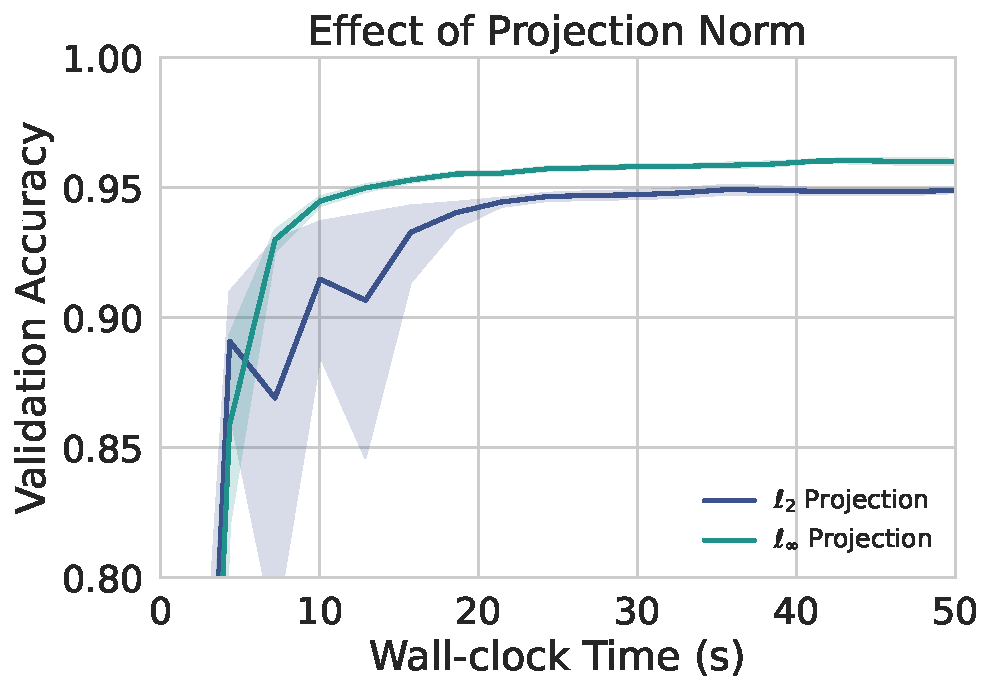
\includegraphics[width=\textwidth]{images/mlp/norm_comparison_time_32.pdf}
        \caption{Batch size 32}
        \label{fig:norm-comparison-32}
    \end{subfigure}
    \hfill
    \begin{subfigure}[t]{0.45\textwidth}
        \centering
        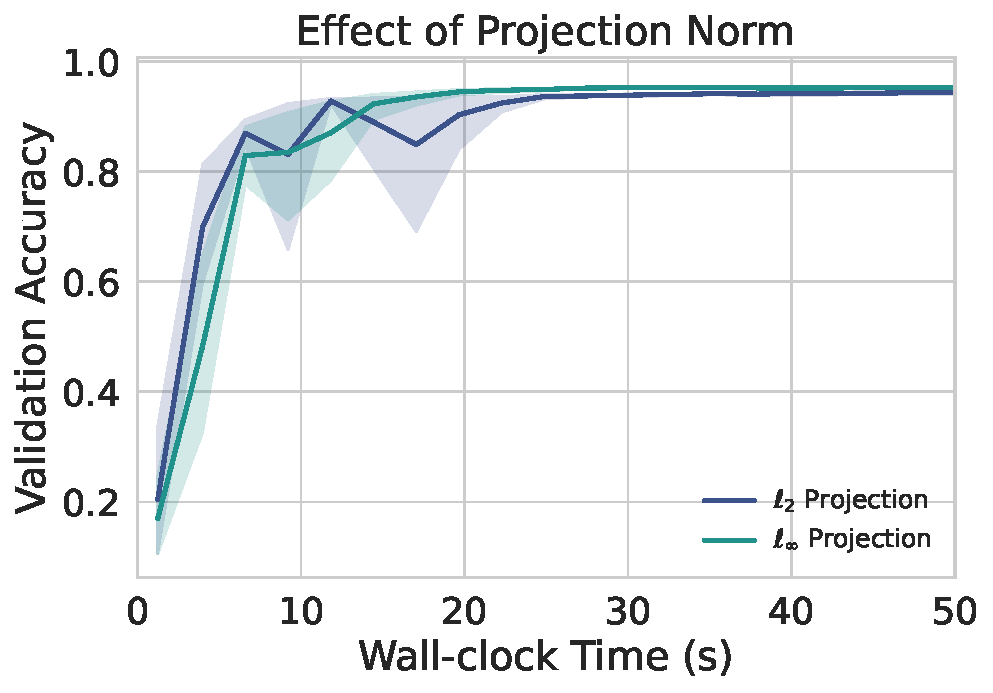
\includegraphics[width=\textwidth]{images/mlp/norm_comparison_time_1024.pdf}
        \caption{Batch size 1024}
        \label{fig:norm-comparison-1024}
    \end{subfigure}
    \caption{Effect of projection norm on validation accuracy over wall-clock time.}
    \label{fig:norm-comparison}
\end{figure}
\\
Empirically, both standard PyTorch and $\mathcal{P}$Torch (configured with an $\ell_2$ projection) scale significantly better and maintain a lower memory baseline than PJAX (\cref{fig:memory}), enabling the training of substantially larger networks before memory exhaustion. This advantage stems from a fundamental difference in asymptotic complexity. $\mathcal{P}$Torch reduces the overhead to $\mathcal{O}(N_{\mathrm{in}}B + N_{\mathrm{out}}B + N_{\mathrm{in}}N_{\mathrm{out}})$, matching the standard asymptotic scaling of PyTorch.
\begin{figure}[ht]
\centering
\safeincludegraphics[width=0.6\textwidth]{images/memory_vs_k.pdf}
\caption{Peak memory versus input dimension for a linear-layer. PJAX scales substantially worse than $\mathcal{P}$Torch and Torch. For small input dimensions, $\mathcal{P}$Torch uses roughly $10\times$ more memory than Torch, but this gap narrows as the input dimension increases.}
\label{fig:memory}
\end{figure}


To get better performance the projections can be fine tuned via the $\alpha$ and $\gamma$ parameters, which dictate whether the weights or activations absorb the majority of the update (\cref{fig:alpha-g-sweep}). Specifically, setting $\gamma \to \infty$ leaves the output values unchanged, whereas setting $\alpha \to  \infty$ leaves the weights unchanged. 
\begin{figure}[ht]
\centering
\begin{subfigure}[t]{0.46\textwidth}
\centering
\safeincludegraphics[width=\textwidth]{images/alpha_g_sweep.png}
\caption{Hyperparameter sweep illustrating the sensitivity to $\alpha$ and $\gamma$.}
\label{fig:matmul-sweep}
\end{subfigure}
\hfill
\begin{subfigure}[t]{0.46\textwidth}
\centering
\safeincludegraphics[width=\textwidth]{images/matmul_projection_sweep_2d.png}
\caption{MatMul projection showing the impact of the tuning parameters.}
\label{fig:alpha-g-sweep}
\end{subfigure}
\label{fig:projection-params}
\end{figure}
In practice, the framework is highly robust and relatively insensitive to these hyperparameters (\cref{fig:matmul-sweep}); however, careful tuning within a reasonable range, typically $[0.01, 500]$, can yield modest gains when maximizing accuracy.

Another tuning parameter for the cyclic projection algorithm is the number of backward passes per data batch. In the current framework, this is fixed at 1, as it allows for a substantially more efficient and elegant implementation. However, this choice may not be optimal, since using multiple backward passes can improve performance per step (\cref{fig:backward-passes}).
\begin{figure}[ht]
\centering
\safeincludegraphics[width=1\textwidth]{images/other_benchmarks/mnist_cyclic_pure_bp_comparison.pdf}
\caption{Error convergence and validation accuracy as a function of the number of backward passes on the MNIST benchmark.}
\label{fig:backward-passes}
\end{figure}


\section{Loss Formulation and Advanced Relaxations}
\label{sec:exp-relaxation-location}
Regarding the loss formulation, replacing the hard target-assignment with a proximal-loss step (\cref{sec:moreau}) accelerates convergence (\cref{fig:effect-of-loss}). Similar benefits to softening the loss constraint have also been reported in prior projection-based literature like PJAX \cite{bergmeister2025projection}.

\begin{figure}[ht]
    \centering
    % Left Figure
    \begin{minipage}{0.45\textwidth}
        \centering
        \safeincludegraphics[width=\textwidth]{images/effect_of_loss.pdf}
        \caption{Replacing hard target-assignment with a proximal-loss step accelerates convergence.}
        \label{fig:effect-of-loss}
    \end{minipage}
    \hfill % Adds horizontal space between the two
    % Right Figure
    \begin{minipage}{0.45\textwidth}
        \centering
        \safeincludegraphics[width=\textwidth]{images/other_benchmarks/xor_activations.pdf}
        \caption{First-order relaxation applied to the hidden states on the XOR benchmark.}
        \label{fig:relaxation-location}
    \end{minipage}
\end{figure}
To further stabilize training, first-order relaxations can also be applied to the projection residuals. Where this relaxation is applied is critical: applying it to both the weight residuals and the hidden states can perform better than applying it to only the weights. Doing this comes with a large memory penalty, as both the hidden states and the weights need to be tracked. To keep the framework simple, we apply relaxation only to the weights by default. However, in some cases, such as the XOR benchmark, applying relaxation more broadly is beneficial (\cref{fig:relaxation-location}).
